\documentclass{beamer}
\usepackage{beamerthemesplit}
\usepackage{graphicx,url}
\usepackage[brazil]{babel}
\usepackage[utf8]{inputenc}
\usepackage{multimedia}

\mode<presentation>
{
  \usetheme{Ilmenau}
  \setbeamercovered{transparent}
}

\newcommand{\eng}[1]{\textit{#1}}
\newcommand{\obra}{\textit{Em torno da romã}}
\newcommand{\goiaba}{\textit{Goiaba}}

\title{\obra{}: aplicações de operações de contorno na composição}
\author{Marcos da Silva Sampaio}
\date{28 de novembro de 2008}

\logo{\includegraphics[scale=.15]{logo-genos}}

\begin{document}

\frame{\titlepage}

\section{Introdução}

\frame{
  \frametitle{O que são contornos?}
  \begin{figure}
    \includegraphics[scale=.6]{roma-pura}
    \hspace{1em}
    \includegraphics[scale=.6]{contorno-com-roma}
  \end{figure}
}

\frame{
  \frametitle{Contornos em Música}
  \vspace{-3em}
  \begin{figure}
    \centering
    \includegraphics{5a-sinfonia}
  \end{figure}

  \href{run:audio/5a-sinfonia.midi}{Tocar}

  \begin{figure}
    \centering
    \includegraphics[scale=1.4]{c-3120}
  \end{figure}
}

\frame{
  \frametitle{Semelhança e possível coerência}
  \begin{figure}
    \centering
    \vspace{-3em}
    \includegraphics{ly-3120-5a-sinfonia}
    \hspace{1em}
    \includegraphics[scale=1.4]{c-3120}
  \end{figure}
  \vspace{-1em}

  \href{run:audio/ly-3120-5a-sinfonia.midi}{Tocar}
}

\frame{
  \frametitle{Possível coerência em Webern}
\begin{figure}
  \centering
    \includegraphics[scale=.7]{webern-tema-analisado}

    \includegraphics[scale=.7]{webern-concatenacao-1}
    \quad
    \includegraphics[scale=.7]{webern-concatenacao-2}
\end{figure}

  \href{run:audio/webern-tema.wav}{Tema}
  \href{run:audio/webern-fragmento-1.wav}{Fr.1}
  \href{run:audio/webern-fragmento-2.wav}{Fr.2}
}


\frame{
  \frametitle{Objetivos e justificativa}
  \begin{itemize}
  \item Justificativa
    \begin{itemize}
    \item Coerência
    \item Manipulação por operações
    \item Estudos escassos
    \end{itemize}
  \item Objetivos
    \begin{itemize}
    \item Composição baseada em operações de contornos
    \item Software para processar contornos
    \end{itemize}
  \end{itemize}
}

\section{Contornos}

\frame{
  \frametitle{Definições}
  \begin{figure}
    \centering
    \includegraphics{5a-sinfonia}
  \end{figure}
  \begin{itemize}
  \item Movimento asc./desc. entre elementos adjacentes

    (- + -)
  \item Conjunto ordenado numerado ascendentemente

    (3 1 2 0)
  \end{itemize}

  \href{run:audio/5a-sinfonia.midi}{Tocar}
}

\frame{
  \frametitle{Comparação entre definições}
  \begin{enumerate}
  \item Elementos não adjacentes
  \item Expansível para outros elementos musicais
  \end{enumerate}

  \vspace{-3em}
  \begin{figure}
    \centering
    \includegraphics[scale=.9]{chord-densities-in-time}
    \hspace{1em}
    \includegraphics[scale=.9]{dynamics-in-time}
    \hspace{1em}
    \includegraphics[scale=1]{c-1023}
  \end{figure}
  \vspace{-2em}

  \href{run:audio/chord.midi}{Tocar acordes}
  \href{run:audio/dynamics.midi}{Tocar dinâmicas}
}

\frame{
  \frametitle{Representações de contornos}
  \begin{itemize}
  \item Representação simbólica

    Contorno: Z(2 0 3 1)
  \item Representação gráfica
    \begin{figure}
      \centering
      \includegraphics[scale=1.5]{c-2031}
    \end{figure}
  \end{itemize}
}

\frame{
  \frametitle{Representação de operações}
  \begin{itemize}
  \item Retrógrado de X(1 2 3):\\
    $retr(X(1\;2\;3))=Y(3\;2\;1)$
  \item Transposição de X(1 2 3) com fator 2: $transp(X(1\;2\;3)\;2)=W(3\;4\;5)$
  \item Concatenação de operações:
    $transp(retr(inv(rot(X(1\;2\;3))\;2))\;3)=K(6\;4\;5)$
  \end{itemize}
}

\frame{
  \frametitle{Operações}
  \begin{itemize}
  \item implementadas no \goiaba{} (rodar no programa)
  \item não implementadas no \goiaba{}
  \end{itemize}
}

\frame{
  \frametitle{Matriz de comparação e INT$_n$}
  \begin{figure}
    \centering
    \begin{tabular}{c|cccc}
      & $5$ & $9$ & $6$ & $8$ \\
      \hline
      $5$ & $0$ & $+$ & $+$ & $+$ \\
      $9$ & $-$ & $0$ & $-$ & $-$ \\
      $6$ & $-$ & $+$ & $0$ & $+$ \\
      $8$ & $-$ & $+$ & $-$ & $0$
    \end{tabular}
  \end{figure}
}

\frame{
  \frametitle{Matriz de comparação e INT$_n$}
  \begin{figure}
    \centering
    \begin{tabular}{c|cccc}
      & $5$ & $9$ & $6$ & $8$ \\
      \hline
      $5$ & $0$ & \textcolor{red}{$+$} & $+$ & $+$ \\
      $9$ & $-$ & $0$ & \textcolor{red}{$-$} & $-$ \\
      $6$ & $-$ & $+$ & $0$ & \textcolor{red}{$+$} \\
      $8$ & $-$ & $+$ & $-$ & $0$
    \end{tabular}
  \end{figure}
}

\frame{
  \frametitle{Matriz de comparação e INT$_n$}
  \begin{figure}
    \centering
    \begin{tabular}{c|cccc}
      & $5$ & $9$ & $6$ & $8$ \\
      \hline
      $5$ & $0$ & $+$ & \textcolor{red}{$+$} & $+$ \\
      $9$ & $-$ & $0$ & $-$ & \textcolor{red}{$-$} \\
      $6$ & $-$ & $+$ & $0$ & $+$ \\
      $8$ & $-$ & $+$ & $-$ & $0$
    \end{tabular}
  \end{figure}
}

\frame{
  \frametitle{Matriz de comparação e INT$_n$}
  \begin{figure}
    \centering
    \begin{tabular}{c|cccc}
      & $5$ & $9$ & $6$ & $8$ \\
      \hline
      $5$ & $0$ & $+$ & $+$ & \textcolor{red}{$+$} \\
      $9$ & $-$ & $0$ & $-$ & $-$ \\
      $6$ & $-$ & $+$ & $0$ & $+$ \\
      $8$ & $-$ & $+$ & $-$ & $0$
    \end{tabular}
  \end{figure}
}

\frame{
  \frametitle{Tipologia de Adams}
  \begin{figure}
    \centering
    \includegraphics[scale=.3]{adams-typology}
  \end{figure}
}

\section{Composição}

\frame{
  \frametitle{Características gerais}
  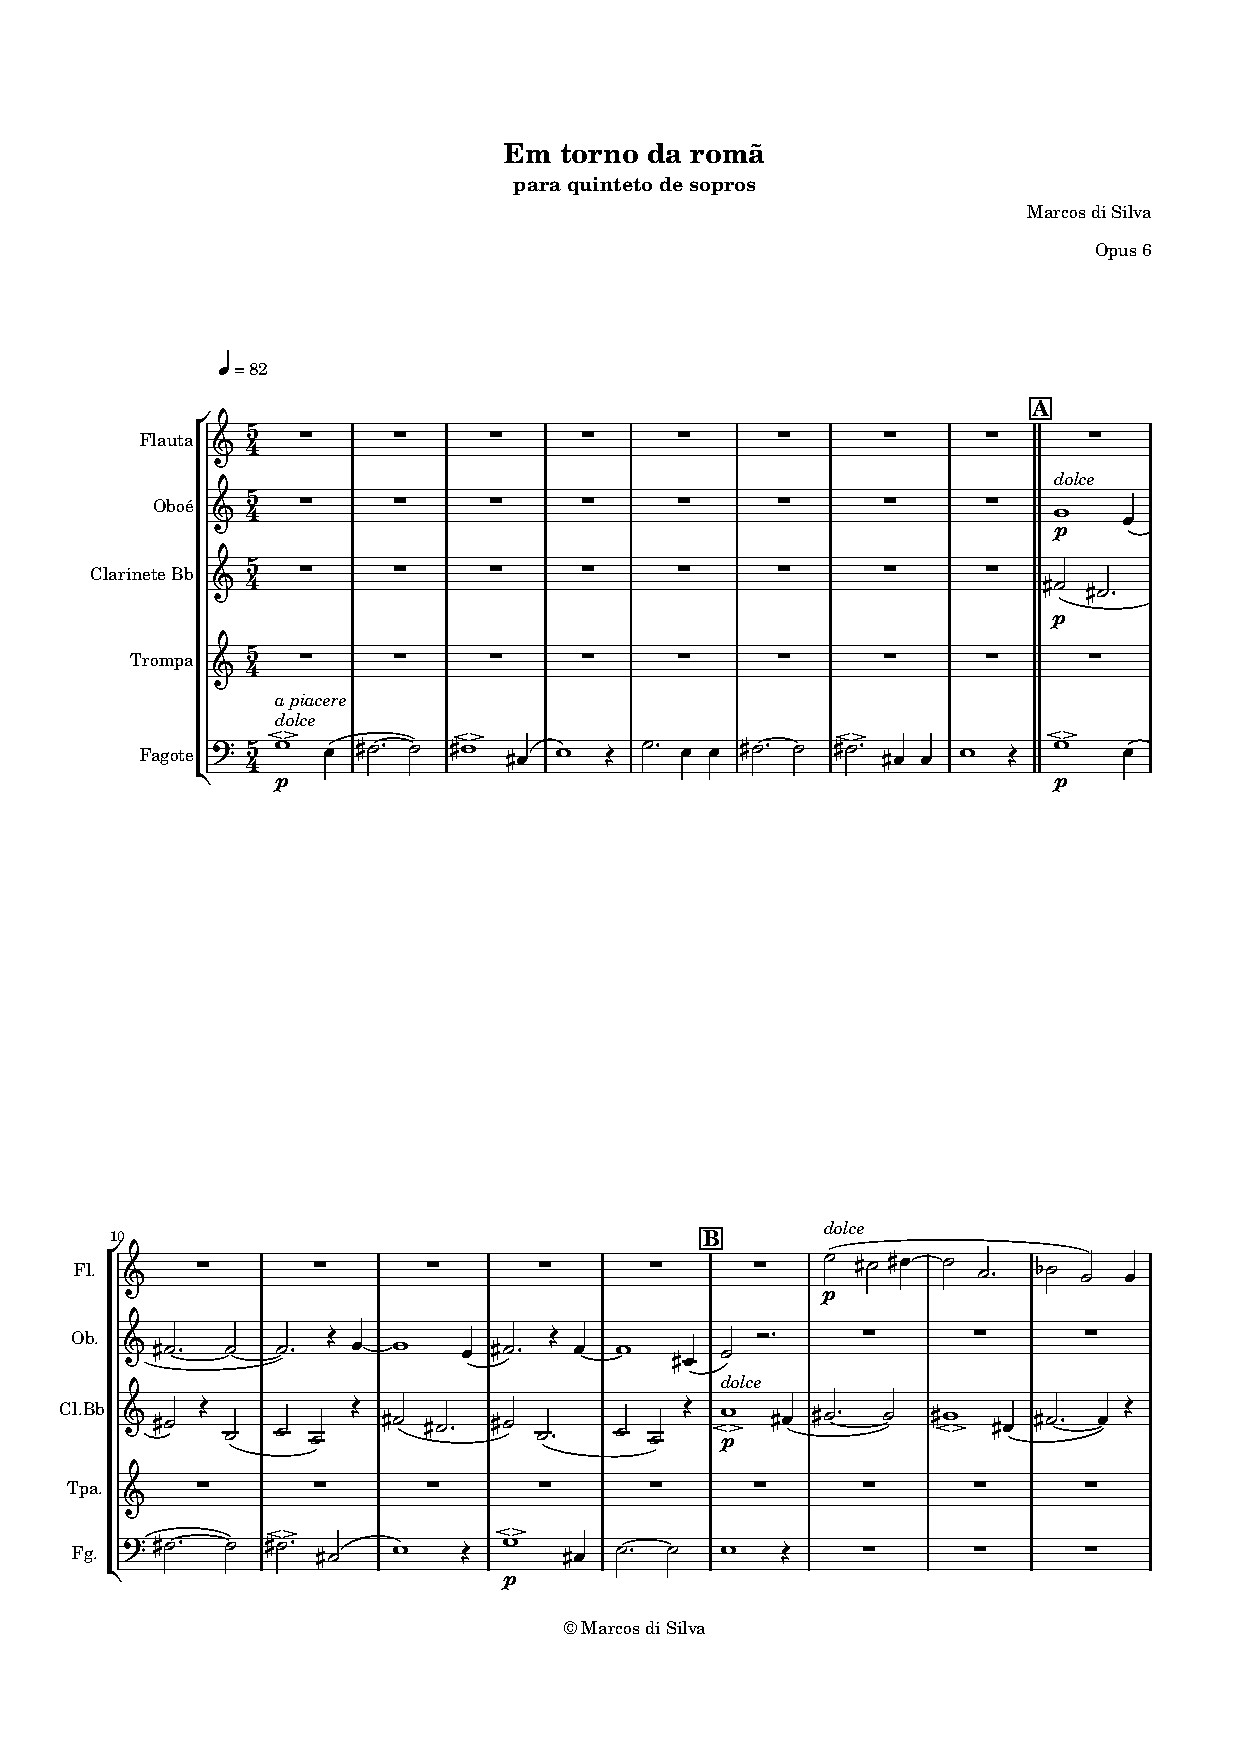
\includegraphics[scale=.55]{pagina-inicial-opus-6}
}

\frame{
  \frametitle{Materiais utilizados}
  \begin{columns}[t]
    \column[T]{4cm}
    \begin{figure}
      \centering
      \includegraphics[scale=1]{motivo-alfa}
      \vspace{-2em}
      \caption{Motivo $\alpha$}
    \end{figure}
    \column{6cm}
    \begin{figure}
      \centering
      \includegraphics[scale=1]{c-534120}
      \caption{Contorno P(5 3 4 1 2 0)}
    \end{figure}
  \end{columns}

  \href{run:audio/motivo-alfa.midi}{Tocar}
}

\frame{
  \frametitle{Uso de motivos}
  \vspace{-4em}
  \begin{columns}
    \hspace{-3em}
    \column{5cm}
    \begin{figure}
      \includegraphics[scale=1]{motivo-alfa-analisado}
      \vspace{-2em}
      \caption{Estrutura do motivo $\alpha$}
    \end{figure}
    \vspace{-4em}
    \begin{figure}
      \includegraphics[scale=.85]{motivo-delta}
      \vspace{-2em}
      \caption{Motivo $\delta$}
    \end{figure}

    \column{4cm}
    \begin{figure}
      \includegraphics[scale=1]{motivo-gama}
      \vspace{-2em}
      \caption{Motivo $\gamma$}
    \end{figure}
    \vspace{-4em}
    \begin{figure}
      \includegraphics[scale=1]{motivo-beta}
      \vspace{-2em}
      \caption{Motivo $\beta$}
    \end{figure}
  \end{columns}
}

\frame{
  \frametitle{Motivos $\alpha$ e $\beta$}
  \hspace{-2em} \includegraphics[scale=.8]{motivos-alfa-e-beta}

  \href{run:audio/ex-motivos-alfa-beta.wav}{Tocar}
}

\frame{
  \frametitle{Motivo $\gamma$}
  \hspace{-2em} \includegraphics[scale=.8]{motivo-gama-na-peca}

  \href{run:audio/ex-motivo-gama.wav}{Tocar}
}

\frame{
  \frametitle{Contorno principal}
  \begin{figure}
    \centering
    \includegraphics[scale=1]{c-534120}
    \caption{Contorno P(5 3 4 1 2 0)}
  \end{figure}
}

\frame{
  \frametitle{Interpolação com expansão}
  \begin{figure}
    \centering
    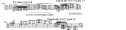
\includegraphics[scale=4.8]{oboe-solo-secao-5}
  \end{figure}

  \href{run:audio/interpolacao-expansao.wav}{Tocar}
}

\frame{
  \frametitle{Rotação com expansão}
  \begin{figure}
    \centering
    \includegraphics[scale=.7]{notas-curtas-madeiras}

    \includegraphics[scale=.55]{c-534120}
    \includegraphics[scale=.55]{c-412053}
    \includegraphics[scale=.55]{c-120534}
    \includegraphics[scale=.55]{c-435021}
  \end{figure}

  \href{run:audio/rotacao-expansao.wav}{Tocar}
}

\frame{
  \frametitle{Rotação com retrogradação}
  \begin{figure}
    \centering
    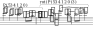
\includegraphics[scale=2.5]{sujeito-fugato}

    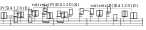
\includegraphics[scale=2.5]{contra-sujeito-fugato}
  \end{figure}

  \href{run:audio/fugato.wav}{Tocar}
  \tiny (mostrar operações no \goiaba{})
}

\frame{
  \frametitle{Expansão associada à amplitude}
  \begin{figure}
    \centering
    \includegraphics[scale=.8]{escala-secao-2-one}
  \end{figure}

  \href{run:audio/escala-secao-2-one.midi}{Tocar}
}

\frame{
  \frametitle{Expansão associada à amplitude}
  \begin{figure}
    \centering
    \includegraphics[scale=.6]{secao-2}
  \end{figure}

  \href{run:audio/secao-2.midi}{Tocar}
}

\frame{
  \frametitle{Expansão associada à amplitude}
  \hspace{-2em} \includegraphics[scale=.7]{lily-044813d1e9-8}

  \href{run:audio/secao-2-completa.wav}{Tocar}
}

\frame{
  \frametitle{Expansão associada à amplitude}
  \hspace{-2em} \includegraphics[scale=.7]{lily-044813d1e9-9}
}

\frame{
  \frametitle{Expansão associada à amplitude}
  \hspace{-2em} \includegraphics[scale=.7]{lily-044813d1e9-10}
}

\frame{
  \frametitle{Expansão associada à amplitude}
  \hspace{-2em} \includegraphics[scale=.7]{lily-044813d1e9-11}
}

\frame{
  \frametitle{Contornos e outros parâmetros}
  \begin{itemize}
  \item Andamentos: 82, 66, 120, 108 e 112. A(1 0 4 2 3)
  \item Densidade. Seção 1: D(1 3 2 5 4)
  \item Complexidade de texturas: (- + - + -)
  \end{itemize}
}

\section{Conclusões}

\frame{
  \frametitle{Conclusões}
  \begin{itemize}
  \item O que foi feito
    \begin{itemize}
    \item Revisão de literatura
    \item Mapeamento de elementos para contornos
    \item Composição de experimentos
    \item Software \goiaba{} $\Longleftarrow$
    \item Composição de \obra{} $\Longleftarrow$
    \end{itemize}
  \item Discussão
    \begin{itemize}
    \item Operações não utilizadas
    \end{itemize}
  \end{itemize}
}

\frame{
  \frametitle{Trabalhos futuros}
  \begin{enumerate}
  \item Teste de outras operações das teorias com pequenos experimentos
  \item Mapeamento de outros parâmetros (dinâmica x densidade)
  \item Uso de contornos em música computacional (outros elementos e parâmetros)
  \item Expansão do software goiaba:
    \begin{itemize}
    \item lançamento de uma versão para usuário
    \item interface gráfica
    \item api fácil de usar
    \item conversão de/para partituras musicais
    \end{itemize}
  \end{enumerate}

  \tiny
  A dissertação está disponível em \url{www.marcosdisilva.net/mestrado}
}

\end{document}
